\section{Our approach}
Next, we describe our approach in implementing the \softner{} framework in detail. As shown in Figure \ref{fig:overview}, we start with the data cleaning process, followed by unsupervised data labeling. Then we describe the label propagation process and the architecture of the deep learning model.

\subsection{Data Cleaning}
Service incident descriptions and summaries are created by various sources such as external customers, feature engineers and even automated monitoring systems. The information could be in various forms, like textual statements, conversations, stack traces, shell scripts, images,  etc., all of which make the information unstructured and hard to interpret. Yet, these descriptions are a goldmine of information, in the form of identifiable entities, amidst other less useful information. Here, we describe the different approaches taken to clean the data before extracting information. First, we prune tables in the incident description that have more than 2 columns and get rid of HTML tags using regexes and HTML parsers. In this process, we also segment the information into sentences using newline characters. Next, we process individual sentences by cleaning up extra spaces and tokenize them into words. Our tokenization technique is able to handle camel-case tokens and URLs as well.

\begin{table*}[!ht]
\small
\caption{Examples of entities extracted by \softner{}}
\vspace{-6pt}
\label{entity-examples}
%\begin{tabular*}{\textwidth}{p{0.2\textwidth}p{0.2\textwidth}p{0.6\textwidth}}
\begin{tabular}{lll}
\toprule
\textbf{Entity Name} & \textbf{Data Type} & \textbf{Example} \\
\midrule
Problem Type & Alphabetical & VNet Failure \\[-1pt]
Exception Message & Alphabetical & The vpn gateway deployment operation failed due to an intermittent error \\[-1pt]
Failed Operation Name & Alphabetical & Create and Mount Volume \\[-1pt]
Resource Id & URI & /resource/2aa3abc0-7986-1abc-a98b-443fd7245e6f/resourcegroups/cs-net/providers/network/frontdoor/ \\[-1pt]
Tenant Id & GUID & 4536dcd6-e2e1-3465-a22b-d25f62456233 \\[-1pt]
Vnet Id & GUID & 45ea1234-123b-7969-adaf-e0255045569e \\[-1pt]
Link With Details & URI & https://supportcenter.cloudx.com/caseoverview?srid=112\\[-1pt]
Device Name & Other & sab01-98cba-1d \\[-1pt]
Source IP & IP Address & 198.168.0.1 \\[-1pt]
Status Code & Numeric & 500 \\[-1pt]
Location & AlphaNumeric & eastus2\\[-1pt]
\bottomrule
\end{tabular}
\end{table*}

\subsection{Unsupervised Data Labelling}
For a lot of tasks in data mining like sentiment classification or even NER, supervised or semi-supervised methods are generally used. However, we don't have any pre-existing labelled data set which can  be used for a supervised NER task. It would also be very expensive to generate labelled data since the entity types vary across different services. So, we have built \softner{} as a completely unsupervised framework. Please refer to Table \ref{entity-examples} for examples of entities extracted using the unsupervised approach. Here are the steps for automatically generating the labelled corpus for named-entity extraction:

\textbf{Step 1 (Entity tagging)}: Since we don't have a list of entity types apriori, we first bootstrap the framework with a candidate set of entity name and value pairs. For this, we have built pattern extractors using the structural patterns commonly used in the incident descriptions: 
\begin{itemize}
    \item \textbf{Key-Value pairs} - This pattern is commonly used in the incident descriptions to specify various entities where the Entity Type and Value are joined by a separator such as ':'. For instance, "\textit{Status code: 401}" or "\textit{Problem type: VM not found}". Here, we split the sentence on the separator and extract the first half as the \textit{Entity Type} and the second half as the \textit{Entity Value}.
    \item \textbf{Tables} - Tables also occur quite frequently in the incident descriptions, especially, the ones which are created by bots or monitoring services. We extract the text in the header tags '\textit{<th>}' as the \textit{Entity Types} and the values in the corresponding rows as the \textit{Entity Values}.
\end{itemize}
 
\textbf{Step 2}: Now, we have a candidate set of entity names and values. However, the candidate set is noisy since we have extracted all the text which satisfies these patterns. In the NER task, entity name corresponds to the category names (for instance, people, location, etc.). So, we filter out any candidates where the entity name contains symbols or numbers. Also, for any NER framework, it's important to have a robust set of named-entities. So, we extract n-grams (n: 1 to 3) from the entity names of the candidates and take the top 100 most frequently occurring n-grams. In this process less frequent, thus noisy candidate entity types, such as \textit{"token acquisition started"}, are pruned. Also with this n-gram analysis, a candidate entity such as [\textit{"My Subscription Id is", "6572"}] would be transformed to [\textit{"Subscription Id", "6572"}] since \textit{"Subscription Id"} is a commonly occurring bi-gram in the candidate set. 

\textbf{Step 3 (Data-type tagging)}: For the refined candidate set, we next infer the data type of the entity values using in-built functions of Python such as "isnumeric" along with regexes. We leverage multi-task learning in \softner{}, where we jointly train the model to predict both the entity type and the data type. These tasks are complementary and help improve the accuracy for the individual prediction tasks. Based on discussions with the service engineers, we have defined the following data types:
\begin{itemize}
    \item \textbf{Basic Types}: Numeric, Boolean, Alphabetical, Alphanumeric, Non-Alphanumeric
    \item \textbf{Complex Types}: GUID, URI, IP Address
    \item \textbf{Other}
\end{itemize}
To infer the data type, we compute it for each instance of a named entity. Then, conflicts are resolved by taking the most frequent type. For instance, if "VM IP" entity is most commonly specified as an IP Address but sometimes is specified as a boolean, due to noise or dummy values, we infer it's data type as an IP Address.

\subsection{Label Propagation}
With the unsupervised tagging, we have bootstrapped the training data using the pattern extraction. While this allows us to generate a seed dataset, the recall would suffer since the entities could occur inline within the incident descriptions without the key-value or tabular patterns. In the absence of ground truth or labeled data, it's a non-trivial problem to solve. In \softner{} we use the unsupervised techniques to label the incident descriptions which are then used to train a deep learning based model. So, to avoid over-fitting the model on the specific patterns, we would want to generalize or diversify the labels.

We use the process of label propagation to solve this challenge. We use the entity values extracted in the bootstrapping process and propagate their types to the entire corpus. For instance, if the IP Address "127.0.0.1" was extracted as a "Source IP" entity, we would tag all un-tagged occurrences of "127.0.0.1" in the corpus as "Source IP". As we can imagine, there are certain edge cases that need to be handled. For instance, we cannot use this technique for entities with Boolean data type. It would also not work for all multi token entities, particularly, the ones which are descriptive. Lastly, it's possible that different occurrences of a particular value were tagged as different entities during bootstrapping. For instance, "127.0.0.1" can be "Source IP" in one incident while "Destination IP" in another incident. We resolve conflicts during label propagation based on popularity, i.e., the value is tagged with the entity type which occurs more frequently across the corpus.

\newcommand{\addREf}{\todo{REF HERE}}

\subsection{\softner{} Deep Learning Model}
\label{sec:multi-task-model}
The previous sections explain the phases of the \softner{} framework, as shown in Figure \ref{fig:overview}, that automate the significant task of creating labeled data for deep learning models which can further generalize knowledge extraction. Here we propose a novel Multi Task deep learning model that solves two entity recognition tasks simultaneously, i.e., Entity Type recognition and Data Type recognition.

The model uses an architecture, as described in Figure \ref{model-arch}, that shares some common parameters and layers for both tasks, but also has task specific layers. Incident descriptions are converted to word level vectors using a pre-trained Glove Embedding layer. This sequence of vectors is interpreted, both forwards and in reverse, by a Bi-directional LSTM layer. We then have distinct layers for the two tasks. The time-distributed layer transposes the BiLSTM hidden vectors to the shape of the output labels and the attention mechanism helps the model bias it's learning towards important sections of the sentences. Finally, the CRF layer produces a valid sequence of output labels. We perform back propagation using a combination of loss functions during training and evaluate individual tag precision, recall and F1 metrics. In the following sub sections we describe the important layers and approaches used in our multi task model.

\subsubsection{\textbf{Word Embeddings}}
\label{sec:glove-word-emb}
Language models in the semantic vector space, require real valued vectors as word representations. The importance of these vectors in improving performance for NLP tasks has been widely studied \cite{collobert2011natural}. These vectors act as characteristic features in applications of language models like question answering, document classification and named entity recognition.
GloVe \cite{pennington2014glove}, introduced a model that captures linear substructure relations in a global corpus of words, revealing regularities in syntax as well as semantics. The GloVe model trained on 5 different corpora, covers a vast range of topics and tokens. GloVe vectors, demonstrated on tasks such as word analogy and named entity recognition in \cite{pennington2014glove}, outperforms various other word representations. To use the 100 dimension version of GloVe, we create an embedding layer with the pre-trained GloVe weights in all our models.

\subsubsection{\textbf{Bi-directional LSTM}}
Recurrent Neural Networks (RNN) have been the basis for numerous language modelling tasks in the past.\cite{mikolov2010recurrent}. An RNN maintains historic information extracted from sequence or series like data. This feature enables RNN based models to make predictions at a certain time step, conditional to the viewed history. They take a sequence of vectors $\boldsymbol{(x_1, x_2, .., x_n)}$ as input and return a sequence of vectors $\boldsymbol{(h_1, h_2, .., h_3)}$ that encodes information at every time step.
Although it can be hypothesized that RNNs are capable of encoding and learning dependencies that are spread over long time steps, evidence shows that they fail to do so. RNNs tend to be biased towards more recent updates in long sequence situations.

Long Short-term Memory (LSTM) networks \cite{hochreiter1997long} were designed to overcome the problems associated with vanilla RNNs. Their architecture allows them to capture long range dependencies using several gates. These gates control the portion of the input to give to the memory cell, and the portion from the previous hidden state to forget. We model the LSTM layer using the following equations:
%
\begin{equation}
    f_{t}=\sigma(W_{f}\cdot[h_{t-1},x_{t}] + b_{f})
\end{equation}
\begin{equation}
    i_{t}=\sigma(W_{i}\cdot[h_{t-1},x_{t}] + b_{i})
\end{equation}
\begin{equation}
    {\tilde {c}}_{t}=\tanh(W_{c}\cdot[h_{t-1},x_{t}] + b_{c})
\end{equation}
\begin{equation}
    c_{t}= f_{t}\circ c_{t-1}+ i_{t}\circ {\tilde {c}}_{t}
\end{equation}
\begin{equation}
    o_{t}=\sigma(W_{o}\cdot[h_{t-1},x_{t}] + b_{o})
\end{equation}
\begin{equation}
    h_{t}=o_{t}\circ \tanh(c_{t})
\end{equation}

In the above equations $\sigma$ is the element wise sigmoid function and the $\circ$ represents hadamard product (element-wise). $f_t, i_t$ and $o_t$ are forget, input, and output gate vectors respectively, and, $c_t$ is the cell state vector. Using the above equations, given a sentence as a sequence of real valued vectors $\boldsymbol{(x_1, x_2, .., x_n)}$, it computes $\overrightarrow{h_{t}}$ that represents the leftward context of the word at the current time step $t$. By intuition, a word at the current time step $t$, receives context from other words that occur on either sides. A representation of this can be achieved with a second LSTM that interprets the same sequence in reverse, returning $\overleftarrow{h_{t}}$ at each time step. This combination of forward and backward LSTM is referred to as Bi-Directional LSTM (BiLSTM) \cite{graves2005framewise}. The final representation of the word is produced by concatenating the left and right context, $h_{t}=[\overrightarrow{h_{t}};\overleftarrow{h_{t}}]$.


\subsubsection{\textbf{Neural Attention Mechanism}}
In recent years attention mechanism has become increasing popular in various NLP applications like neural machine translation \cite{bahdanau2014neural}, sentiment classification \cite{chen2017recurrent} and parsing \cite{li2016discourse}. Novel architectures like transformers \cite{vaswani2017attention} and BERT \cite{devlin2018bert} have proven the effectiveness of such a mechanism for various downstream tasks. In addition to the improvements BiLSTMs bring to the original RNN approach, attention mechanism addresses long input sequences by retaining and utilising all hidden states generated. We implement attention at the word level as a neural layer, with a weight parameter $W_{a}$. It takes as input the the hidden states from the BiLSTM, transposed to output dimensions using a time distributed dense layer. Let $h = [h_1, h_2, .. h_{T}]$ be the input to the attention layer. The attention weights and final representation $h^*$ of the sentence is formed as follows:
\begin{equation}
    scores = W_a^Th
\end{equation}
\begin{equation}\label{attention-score}
    \alpha = softmax(scores)      
\end{equation}
\begin{equation}
    r = h\alpha^T    
\end{equation}
\begin{equation}\label{attention-repr}
    h^* = \tanh(r)    
\end{equation}

In equations \ref{attention-score} \& \ref{attention-repr} the $softmax$ and $tanh$ functions are applied element-wise on the input vectors. We then concatenate $h$ and $h^*$ and pass it to the next layer. We visualize the attention vector $\alpha$ for a test sentence in Figure \ref{attention-viz}, where we observe that the attention layer learns to give more emphasis to tokens that have a higher likelihood of being entities. In Figure \ref{attention-viz}, the darkness in the shade of blue is proportional to the degree of attention. In case of long sequences, this weighted attention to certain sections of the sequence, that are more likely to contain entities, helps improve the model's sensitivity\footnote{Sensitivity, also known as recall, is the proportion of actual positives that are correctly identified}.

\begin{figure}%[H]
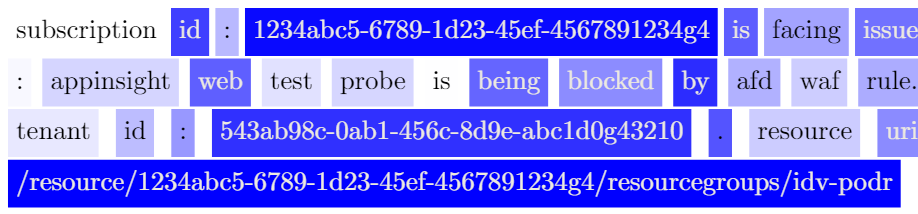
\includegraphics[width=\linewidth]{Figures/attention_viz.png}
\vspace{-12pt}
\caption{Attention visualization on a sample input}
\label{attention-viz}
\vspace{-6pt}
\end{figure}

\subsubsection{\textbf{Conditional Random Fields}}
A simple approach to sequence tagging with LSTMs is to use the hidden state representations ($h_t$) as word features to make independent tagging decisions at the word level. But that leaves behind inherent dependencies across output labels in tasks like Named Entity Recognition. Our NER task also has this characteristic since the initial \softner{} heuristics enforce structural constraints, for example, separators between key-value and html table tags. In learning these dependencies and generalizing them to sentences without these constraints, we model tagging decisions jointly using conditional random fields 
\cite{lafferty2001conditional}.

For an input sequence $\boldsymbol{X = (x_1, x_2, .., x_n)}$, let $\boldsymbol{y = (y_1, y_2, .., y_n)}$ a potential output sequence, where n is the no of words in the sentence. Let $P$, the output of the BiLSTM network passed through the dense and attention layers, be the matrix of probability scores of shape $n \times k$, where k is the number of distinct tags. That is $P_{i,j}$ is a score that the $i^{th}$ word corresponds to the $j^{th}$ tag. We define CRF as a layer in the model, whose working is as follows. First a score is computed for $y$.

\begin{equation}
    s(\boldsymbol{X,y}) = \sum_{i=0}^{n} A_{y_i,y_{i+1}} + \sum_{i=0}^{n} P_{i,y_{i}} 
\end{equation}

where A represents the matrix of transition scores. That is $A_{i,j}$ is the score for the transition from $tag_i$ to $tag_j$. Then the score is converted to a probability for the sequence $y$ to be the right output using a softmax over $\boldsymbol{Y}$(all possible output sequences). 

\begin{equation}
    p(\boldsymbol{y|X}) = 
    \dfrac{e^{s(\boldsymbol{X,y})}}{\sum_{y' \in Y} e^{s(\boldsymbol{X,y'})}  }
\end{equation}

The model learns by maximizing the log-probability of the correct $y$. While extracting the tags for the input, we predict the output sequence with the highest score.

\begin{equation}
    \boldsymbol{y^*} = \argmax_{y' \in Y} p(y'|X)
\end{equation}

From the above implementation it is clear as to how the CRF and attention layers push the model towards learning a valid sequence of tags, unlike in the case of independent tagging as discussed.

\begin{figure}%[H]
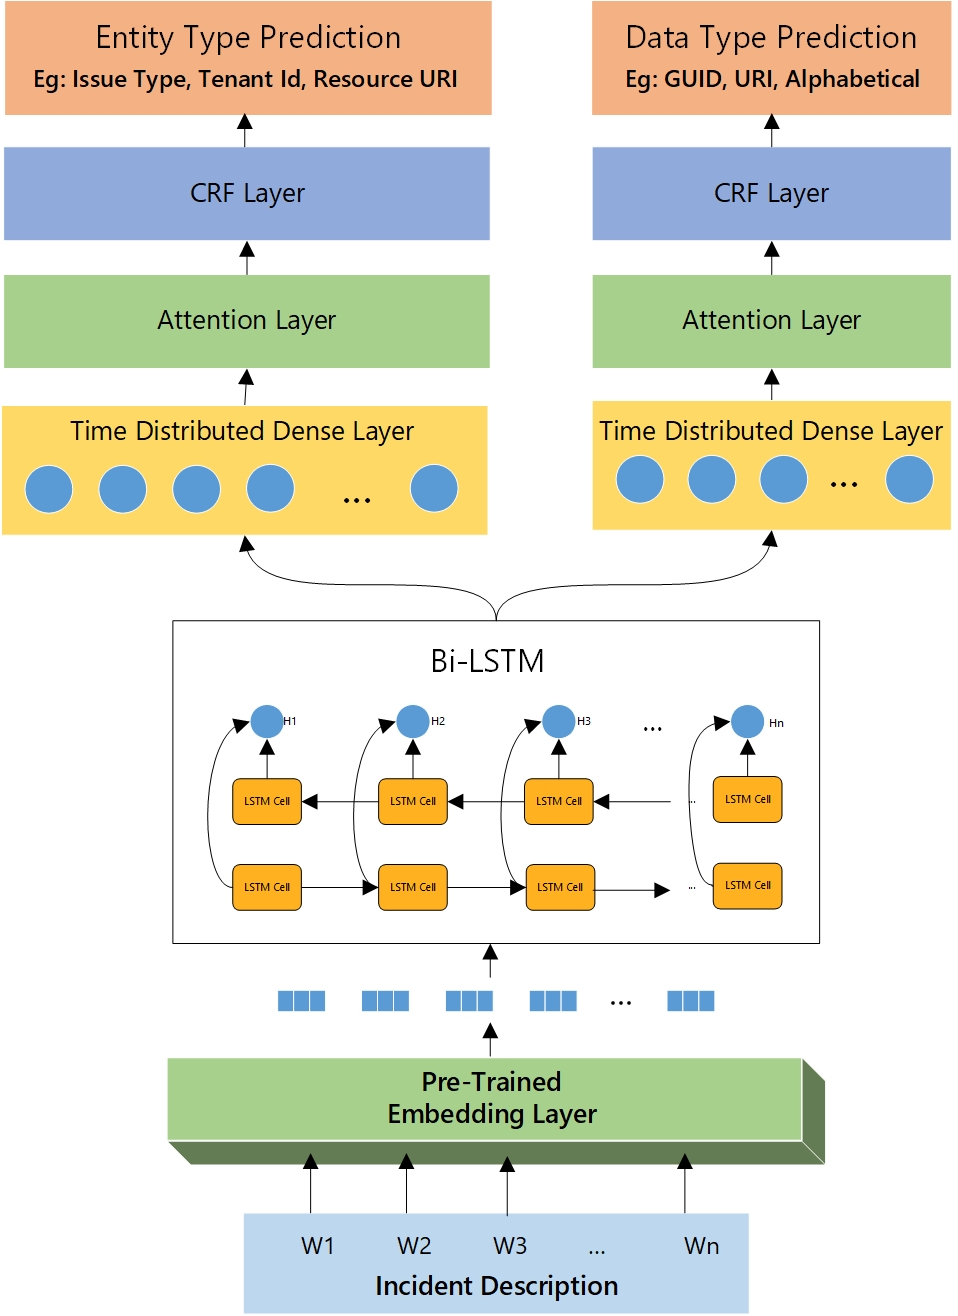
\includegraphics[width=\linewidth]{Figures/MTL_Diagram.jpg}
\caption{Multi-task model architecture}
\label{model-arch}
%\vspace{-6pt}
\end{figure}

\subsubsection{\textbf{Multi-Task Learning}}

Caruana et al. \cite{caruana1997multitask} defines Multi-Task Learning (MTL) as an approach to improve generalization in models by using the underlying common information contained among related tasks. Some well known applications for MTL are multi-class and multi-label classification problems. In the context of classification or sequence labelling, MTL improves the performance of individual tasks by learning them jointly.

In \softner{}, named-entity recognition is the primary task. In this task, models mainly learn from context words that support occurrences of entities. But we also observe that incorporating a complimentary task of predicting the data-type of a token reinforces intuitive constraints, indirectly to model training. For example in an input like "\textit{The SourceIPAddress is 127.0.0.1}", the token \textit{127.0.0.1} is identified more accurately by our model, as the entity type "\textbf{Source Ip Address}", because it is also identified as the data-type "\textbf{Ip Address}", in parallel. This supplements the intuition that all \textit{Source Ip Addresses} are \textit{Ip adresses}, thus, improving model performance. Therefore, we choose data type prediction as the auxiliary task for \softner{}'s deep learning model.

There are multiple architectures that allow multi-task learning, like Multi-head architecture, Cross-snitch Networks\cite{misra2016cross} and Sluice Networks \cite{ruder2017learning}. We use the Multi-head architecture, where the lower level features generated by the BiLSTM layers are shared, whereas the other layers are task specific. The combined architecture is depicted in Figure \ref{model-arch}. As stated above, we define the entity type prediction as the main task and that of data type prediction as the auxiliary task. The losses are initially calculated individually for both tasks, $l_1$ and $l_2$, and then combined into $loss_{c}$ using a weighted sum. The parameter $loss\_weights = (\alpha,\beta)$ is used to control the importance between main and auxiliary task as follows:

\begin{equation}
    loss_{c} = \alpha \times l_1 + \beta \times l_2
\end{equation}

During training, the model aims to minimize the $loss_{c}$ but the individual losses are back-propagated to only those layers that produced the output. With such an approach, the lower level common layers are trained by both tasks, whereas the task specific layers are trained by individual losses.

\subsection{Implementation}

We implement \softner{} and all the machine learning models using Python 3.7.5, with Keras-2.2.4 and the tensorflow-1.15.0 backend. The hyper-parameters for the deep learning models are set as follows: word embedding size is set to 100, hidden LSTM layer size is set to 200 cells, and, maximum length of a sequence is limited to 300. These hyper-parameters were re-used among all models. The embedding layer uses pre-trained weights from glove.6B.100d, downloaded from the official stanford-nlp website\footnote{http://nlp.stanford.edu/data/glove.6B.zip}. Our models are trained on an Ubuntu 16.04 LTS machine, with 24-core Intel Xeon E5-2690 v3 CPU (2.60GHz), 112 GB memory and 64-bit operating system. The machine also has a Nvidia Tesla P100 GPU with 16 GB RAM.

We have also deployed \softner{} as a REST API developed using the Python Flask web app framework. The REST API offers a POST endpoint which takes the incident description as input and returns the extracted entities in JSON format. We have deployed it on the cloud platform provided by \CompanyX{} which allows us to automatically scale the service based on the variation in request volume. This enables the service to be cost efficient since majority of the incidents are created during the day. We have also enabled application monitoring which alerts us in case the availability or the latency regresses.